\documentclass[11pt,letterpaper]{article}

\usepackage[T1]{fontenc}
\usepackage{lmodern}
\usepackage[margin=1in]{geometry}
\usepackage{amsmath,amssymb,amsthm}
\usepackage{booktabs}
\usepackage{array,tabularx}
\usepackage{float}
\usepackage{xcolor}
\usepackage{colortbl}
\usepackage{xurl}
\usepackage{microtype}
\usepackage{xspace}
\usepackage{enumitem}
\usepackage{tikz}
\usepackage{graphicx}
\usetikzlibrary{arrows.meta,positioning,fit,calc}
\usepackage[hidelinks]{hyperref}
\usepackage[nameinlink,noabbrev]{cleveref}
\emergencystretch=2em
\allowdisplaybreaks

\newtheorem{theorem}{Theorem}[section]
\newtheorem{lemma}[theorem]{Lemma}
\newtheorem{proposition}[theorem]{Proposition}
\theoremstyle{definition}
\newtheorem{definition}[theorem]{Definition}
\theoremstyle{remark}
\newtheorem{remark}[theorem]{Remark}

\newcommand{\scheme}{\ensuremath{\mathsf{CipherAuth}}\xspace}
\newcommand{\CEA}{\ensuremath{\mathsf{CEA}}\xspace}
\newcommand{\Adv}{\ensuremath{\mathsf{Adv}}}
\newcommand{\Succ}{\ensuremath{\mathsf{Succ}}}
\newcommand{\GClass}{\ensuremath{\mathsf{G\text{-}CONF\text{-}CLASS}}\xspace}
\newcommand{\GCT}{\ensuremath{\mathsf{G\text{-}CONF\text{-}CT}}\xspace}
\newcommand{\GScope}{\ensuremath{\mathsf{G\text{-}SCOPE}}\xspace}
\newcommand{\Zq}{\ensuremath{\mathbb{Z}_q}}
\newcommand{\RO}{\ensuremath{\mathcal{H}}}
\newcommand{\KeyRef}{\ensuremath{\mathsf{KeyRef}}}
\newcommand{\KDF}{\ensuremath{\mathsf{KDF}}}
\newcommand{\Hd}{\ensuremath{H_{\mathsf d}}}
\newcommand{\Hc}{\ensuremath{H_{\mathsf c}}}
\newcommand{\Hmask}{\ensuremath{H_{\mathsf{mask}}}}
\newcommand{\HOmega}{\ensuremath{H_{\Omega}}}
\newcommand{\ReEncO}{\ensuremath{\mathsf{ReEncO}}}
\newcommand{\DecO}{\ensuremath{\mathsf{DecO}}}
\newcommand{\GrantO}{\ensuremath{\mathsf{GrantO}}}
\newcommand{\TEST}{\ensuremath{\mathsf{TEST}}}
\newcommand{\artifacturl}{\url{https://anonymous.4open.science/r/CipherAuth-7A03/README.md}}
\newcolumntype{Y}{>{\raggedright\arraybackslash}X}

\title{Aggregate Authentication under Proxy Re-encryption:\\
A Security Boundary between Ciphertext- and Class-Granular Confidentiality}
\author{\textbf{Anonymous manuscript for review}}
\date{}

\begin{document}
\pagenumbering{gobble}
\begin{titlepage}
\maketitle

\begin{abstract}
Encrypted collection systems may need to compress authentication before a proxy
delegates decryption to a new recipient.  A direct composition is difficult:
aggregate authentication normally binds the ciphertext transcript, whereas
proxy re-encryption changes that transcript.  We study a commit--encrypt--
aggregate--delegate comparator in which each sender signs a commitment to its
message, Schnorr responses are half-aggregated, and the proxy changes only the
encryption point.  Aggregation and delegation then commute exactly.  This
identity follows from the invariant signed statement and supplies the functional
baseline for the security analysis.

The same design exposes a confidentiality boundary.  Public aggregate
verification does not validate the encryption point.  A corrupt delegatee can
shift the challenge point, obtain one permitted transformation, remove the known
shift, and recover the challenge opening.  The attack wins a natural
ciphertext-granular game with advantage one and uses neither a hash collision nor
a decryption-oracle query.  We therefore separate ciphertext granularity from a
weaker class-granular game that refuses every target-class transformation to a
corrupt recipient.  The latter notion is strictly weaker than honest-
reencryption-attack security.

For the class-granular game, we give a candidate random-oracle reduction under a
gap variant of Divisible Computational Diffie--Hellman.  Its central simulation
samples the scalar proxy token directly after a uniform-mask hybrid, which
eliminates the algebraic extraction premise required by an earlier proof route.
The bound accounts explicitly for honest delegatees, proof-hash prequeries,
commitment queries, and decryption attempts.  Independent class keys give an
exact fixed-target scope composition.  An executable artifact fixes the games,
encodings, attack, and hybrid bookkeeping; its 286 unique tests and 33
deterministic trace replays pass without failures or skips.
\medskip
\noindent\textbf{Keywords:} proxy re-encryption; aggregate signatures;
signcryption; chosen-ciphertext security; random-oracle model.
\end{abstract}
\end{titlepage}

\pagenumbering{roman}
\tableofcontents
\clearpage
\pagenumbering{arabic}

\paragraph{Proof status.}
The theorem statements in
Sections~\ref{sec:class-proof} and~\ref{sec:scope} are candidate results until a
cryptographer independently checks every oracle simulation and loss term.  The
negative result in Section~\ref{sec:attack} and the exact identities in
Sections~\ref{sec:construction} and~\ref{sec:attack} are algebraic and are covered
by executable tests.

\section{Introduction}

Data collection systems often need three operations at once.  Many senders
produce encrypted records, an intermediary compresses their authentication, and
a proxy later delegates decryption to another recipient without learning the
messages.  A direct combination is fragile.  Aggregate authenticators tend to
bind the ciphertext transcript, while proxy re-encryption changes that transcript.
Removing the changing term from the authenticator can restore commutation but can
also create a receiver-insider forgery.

The syntactic conflict can be resolved by committing to the plaintext,
encrypt it, sign the commitment rather than the ciphertext, and aggregate the
signatures.  The signed statement is then invariant under delegation.  This idea
combines signcryption and joint signature--encryption
disciplines~\cite{Zheng97,ADR02}, single-hop proxy re-encryption constructions
and security models~\cite{BBS98,AFGH06,CH07}, and incremental half-aggregation
of Schnorr signatures~\cite{CGKN21,CZ22}.  We call the resulting comparator \CEA.  The
name is descriptive: it denotes commit, encrypt, and authenticate.

Exact commutation does not settle confidentiality.  In \CEA, public verification
authenticates the message commitment, not the encryption point.  This distinction
is harmless for an origin recipient, who checks the commitment after decryption.
It is harmful for a proxy that must decide whether a submitted ciphertext may be
transformed.  A shifted encryption point retains a valid aggregate authenticator,
and the shift survives proxy transformation in a form that a corrupted delegatee
can remove.  Thus a construction may have correct delegation, authentic origin
statements, and exact aggregate commutation while failing a natural
per-ciphertext proxy security game.

This paper separates the two confidentiality levels.  The stronger notion,
\GCT, permits the honest proxy to serve nonderivative target-class ciphertexts to
a corrupted delegatee.  We show that \CEA fails this notion with advantage one.
The weaker notion, \GClass, treats the independently keyed class---an origin,
tag, and epoch---as the authorization boundary.  It never serves that target
class to a corrupted party.  The distinction matches the construction: a
proxy--delegatee coalition can recover the class key, making the class itself the
authorization unit.

\subsection{Contributions}

Our first contribution is a precise negative result.  We give an algebraic
\(A\)-mauling attack against \GCT.  The attack changes only an encryption point,
passes public aggregate verification, and uses one permitted proxy query to
recover the challenge opening.  The attack is purely algebraic and applies to
the specified construction independently of implementation details.

Second, we freeze a class-granular game and give a candidate quantitative
reduction.  The main technical correction is type-level but consequential.  The
proxy secret \(\Omega=\omega k\) is a scalar, not the point \(\omega K\).  After a
random-oracle hybrid makes the token mask uniform, a simulator can sample
\(\Omega\) directly and answer every honest-delegatee transform exactly as
\(\bar A=\Omega^{-1}A\), using only the sampled proxy scalar.  A separate gap-DCDH
reduction accounts for exposure of the masked token point.

Third, we show that independently keyed non-target classes compose exactly with
the class theorem.  For a target fixed before setup, the resulting \GScope game
preserves the same assumption and bound.  Adaptive target selection,
in-class proxy--delegatee collusion, revocation, and concrete-hash analysis form
separate security questions.

Finally, we supply a reproducible artifact.  It includes the frozen game
interfaces, canonical encodings, the attack, hybrid probes, and a complete
sender-to-delegatee execution.  Tests establish functional and algebraic claims;
the computational claims rest on the accompanying reductions.

Taken together, these results identify the security boundary of invariant
commitment authentication under proxy transformation: ciphertext-granular
confidentiality fails by a concrete algebraic attack, whereas class-granular
confidentiality admits an explicit candidate bound.  This separation, rather
than the commutation identity alone, is the paper's central contribution.

\section{Related work and positioning}
\label{sec:related}

\paragraph{Proxy re-encryption and the security hierarchy.}
Early PRE schemes established bidirectional and unidirectional delegation
mechanisms~\cite{BBS98,AFGH06}; Canetti and Hohenberger then formalized
chosen-ciphertext-secure PRE, including derivative restrictions and key
registration issues~\cite{CH07}.  Replayable CCA security masks challenge-equal
outputs rather than rejecting every related ciphertext, a pattern used by our
decryption rule~\cite{CKN03}.  More recent work argues that CPA is too weak for
PRE and introduces honest-reencryption-attack (HRA) security, which permits
honest reencryption from an honest delegator to a corrupt recipient
~\cite{Cohen19}.  Tight and adaptively secure HRA constructions now exist in the
standard model~\cite{CohenEtAl25,LingEtAl25}.  This hierarchy is essential for
interpreting our result: \GCT permits proxy service on adversarially modified,
nonderivative target ciphertexts to a corrupt delegatee and is therefore
CCA-like and stronger than HRA in this respect; \GClass refuses all target-class
service to corrupt recipients and is intentionally weaker than HRA.  This
placement makes \CEA a comparator for the granularity boundary studied here.

\paragraph{Joint authentication and encryption.}
Signcryption originates with Zheng~\cite{Zheng97}.  An, Dodis, and Rabin show
that natural signature--encryption compositions require careful joint security
definitions~\cite{ADR02}.  Fuchsbauer, Plouviez, and Seurin prove
Schnorr-signed ElGamal CCA security in the algebraic group and random-oracle
models~\cite{FPS20}.  Their public proof of encryption randomness motivates a
repair for our mauling attack, but a compressed multi-record repair would still
need per-record knowledge soundness.  Signatures on randomizable ciphertexts
instead authenticate a plaintext-equivalence class across rerandomization
~\cite{BF20}; their transformation scope is rerandomization rather than
recipient-changing PRE.

\paragraph{Aggregate authentication.}
Pairing-based aggregate signatures achieve compact aggregation
~\cite{BGLS03}.  For Schnorr-type signatures, noninteractive half aggregation
compresses the response scalars while retaining the commitment points
~\cite{CGKN21}.  Chen and Zhao give a tight AGM--ROM analysis and an incremental
construction~\cite{CZ22}.  Recent alternatives occupy different points in the
design space: DahLIAS gives two-round, constant-size, pairing-free aggregation
under an algebraic one-more-DL assumption~\cite{NRS26}; transcript rebinding
amortizes interactive transcripts across signing domains~\cite{ZWL26}; and
plain-model constant-size aggregation is known with pairings and a long setup
~\cite{HWW25}.  These works supply the authentication compressors against which
our proxy-validity boundary is defined.

\paragraph{Closest combined functionality.}
The closest application-level overlap is the pairing-based identity-based
aggregate signcryption with re-encryption scheme of Choi, Jeong, and
Byun~\cite{CJB26}.  There, a UAV verifies and decrypts sensor reports before
aggregate re-encryption to a base station.  In \CEA, the proxy remains
plaintext-oblivious and the main question is which authentication facts survive
an algebraic transform.  Table~\ref{tab:position} locates that question across
the adjacent PRE, signcryption, and aggregation literatures.

\begin{table}[t]
\centering
\caption{Comparison with the principal lines of related work.  ``External''
means that authentication is not integrated into the re-encryption transform.
The final column isolates the security or trust boundary most relevant to this
paper.}
\label{tab:position}
\scriptsize
\setlength{\tabcolsep}{2.7pt}
\renewcommand{\arraystretch}{1.12}
\rowcolors{2}{gray!5}{white}
\begin{tabularx}{\textwidth}{p{0.145\textwidth}p{0.12\textwidth}p{0.15\textwidth}p{0.12\textwidth}p{0.105\textwidth}Y}
\toprule
Work & Ciphertext transform & Authenticated object & Aggregation & Proxy sees plaintext & Security or trust boundary \\
\midrule
BBS PRE~\cite{BBS98} & recipient change & external & none & no & Foundational atomic PRE; predates modern CCA and HRA notions. \\
Unidirectional PRE~\cite{AFGH06} & recipient change & external & none & no & Storage-oriented delegation; no aggregate authentication. \\
CCA PRE~\cite{CH07} & recipient change & external & none & no & Derivative-aware chosen-ciphertext security. \\
Unidirectional CCA PRE~\cite{LV08} & recipient change & external & none & no & Strong classical PRE baseline; pairing-based. \\
HRA PRE~\cite{Cohen19} & honest reencryption & external & none & no & Corrupt recipient may receive an honest reencryption. \\
Tight HRA PRE~\cite{CohenEtAl25,LingEtAl25} & recipient change & external & none & no & Tight or adaptive multi-challenge HRA security. \\
Joint signature and encryption~\cite{ADR02,FPS20} & none & ciphertext or committed message & none & --- & Joint authenticity and confidentiality; no delegation. \\
Randomizable-ciphertext signatures~\cite{BF20} & rerandomize & plaintext equivalence class & none & no & Authentication adapts to rerandomization, not recipient change. \\
Pairing aggregates~\cite{BGLS03,HWW25} & none & signed messages & constant-size & --- & Pairing-based aggregation in the ROM or plain model. \\
Schnorr half aggregation~\cite{CGKN21,CZ22} & none & Schnorr statements & one scalar plus commitments & --- & Authentication compression independent of PRE validity. \\
Interactive DL aggregation~\cite{NRS26,ZWL26} & none & interactive or rebound transcripts & constant-size or domain-scaled & --- & Requires interaction or certified transcript rebinding. \\
ID aggregate signcryption/PRE~\cite{CJB26} & UAV-mediated recipient change & sensor signcryptions & aggregate signcryption & yes & The UAV verifies and decrypts reports before re-encryption. \\
\rowcolor{blue!5}\CEA (this work) & recipient change & invariant commitment & Schnorr half aggregation & no & Separates the \GCT attack from the candidate \GClass bound. \\
\bottomrule
\end{tabularx}
\rowcolors{2}{}{}
\end{table}

\section{Model and notation}
\label{sec:model}

Let \(G\) be a cyclic additive group of prime order \(q\), generated by \(P\).
All externally supplied points are validated, the identity is rejected where the
algorithm requires a nonzero point, and scalars are canonically encoded in
\([0,q)\).  The implementation instantiates \(G\) with P-256 and SHA-256 with
rejection sampling; the security analysis is stated in the random-oracle model.

A key reference is a tuple
\[
  \KeyRef=(\mathsf{id},\mathsf{role},\mathsf{version},\mathsf{fingerprint}).
\]
An origin class is the full origin decryption-key reference together with a tag
\(\tau\) and epoch \(e\).  Class keys are independent.  A sender has Schnorr key
\(x_S\) and public key \(X_S=x_SP\).  An origin class has decryption secret \(k\)
and public key \(K=kP\).  A delegatee \(\ell\) has secret \(k_\ell\) and public
key \(K_\ell=k_\ell P\).

Registration accepts adversarial group elements under identities controlled by
the adversary.  Registration is nonextracting and omits proof of possession.
The identity layer is assumed to prevent an adversary from registering a new key
version for an honest identity.  Corruptions are static in the confidentiality
games considered here.

The oracles \(\Hd\), \(\Hc\), \(\KDF\), \(\Hmask\), and \(\HOmega\) are
domain-separated.  Hash inputs use typed, length-delimited encodings.  The symbol
\(\lambda\) denotes the bit length of message-opening digests and commitments;
the implementation uses \(\lambda=256\).

\paragraph{Gap divisible computational Diffie--Hellman.}
The named assumption used below gives a solver an instance
\((P,U=aP,V=bP)\), for independent nonzero \(a,b\), and a decision oracle that
returns one precisely when \(Y=aX\) for a submitted pair \((X,Y)\).  The task is
to output \((b/a)P\).  The game adversary never receives the decision oracle.
The output problem is the Divisible Computational Diffie--Hellman (DCDH)
problem, shown equivalent to computational, inverse, and square CDH in the
high-granularity sense~\cite{BaoDengZhu03}.  The additional fixed-key decision
oracle makes the exact interface a gap-DCDH variant; the artifact retains the
label GDivDH for reproducibility.

\section{The commit--encrypt--aggregate--delegate comparator}
\label{sec:construction}

Figure~\ref{fig:protocol-boundary} separates the three data lanes that matter
for the security analysis.  The aggregate authenticator binds the canonical
statement containing \(c\); the payload \(E\) is checked only after opening; and
the proxy changes the unsigned point \(A\).  The last lane makes delegation
possible and is also the source of the point-shifting attack.

\begin{figure}[H]
\centering
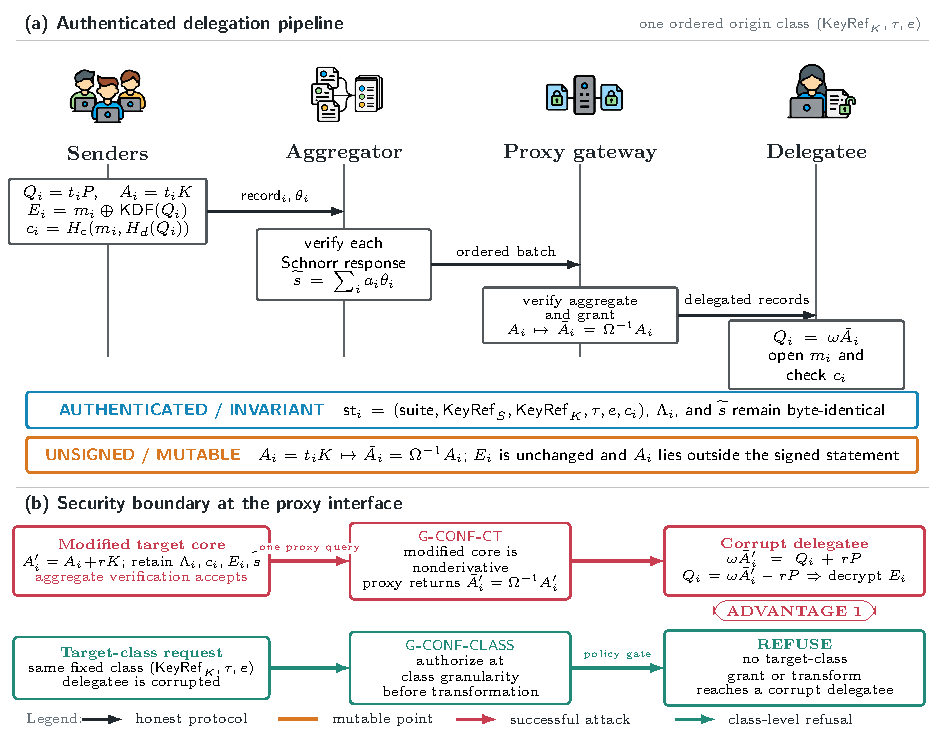
\includegraphics[width=\textwidth]{figures/cipherauth_figure1.pdf}
\caption{CipherAuth dataflow and its security boundary.  Delegation preserves
the commitment-bound aggregate statement exactly, but the proxy-validity
decision depends on an unsigned, algebraically mutable point.  The red path is
the one-query attack against ciphertext-granular confidentiality; the weaker
class-granular game refuses this service to corrupt target recipients.}
\label{fig:protocol-boundary}
\end{figure}

\subsection{Origin records}

To encrypt a message \(m\) for class key \(K=kP\), a sender samples
\(t\leftarrow\Zq^*\) and computes
\begin{align*}
  Q&=tP, & A&=tK, & d&=\Hd(Q),\\
  E&=m\oplus\KDF(Q,|m|), & c&=\Hc(m,d). &&
\end{align*}
The authenticated statement is the canonical encoding
\[
  \mathsf{st}=\mathsf{enc}(\mathsf{suite},\KeyRef_S,\KeyRef_K,\tau,e,c).
\]
The sender produces a Schnorr signature \((\Lambda,\theta)\)~\cite{Schnorr91} on
\(\mathsf{st}\).  The record body contains \((\Lambda,c,A,E)\); the individual
response \(\theta\) is supplied to the aggregator but is omitted from the final
compressed object.

For an ordered sequence, the aggregator verifies every individual signature and
uses the Chen--Zhao prefix-coefficient form
\[
 a_1=1,\qquad
 a_i=H_2((\Lambda_1,X_1,\mathsf{st}_1),\ldots,
          (\Lambda_i,X_i,\mathsf{st}_i))\quad(i\ge2),
\]
with nonzero coefficients where required by the transcript.  It publishes the
records and the scalar
\(\widetilde s=\sum_i a_i\theta_i\).  Public verification recomputes the full
ordered transcript and checks the corresponding aggregate Schnorr equation.

\subsection{Grants and delegation}

For a grant from class \(K=kP\) to delegatee \(K_\ell=k_\ell P\), the origin
samples \(\omega,t'\leftarrow\Zq^*\) and computes
\begin{align*}
 T&=t'P, &
 C&=\mathsf{enc}(\omega)\oplus\Hmask(T,\KeyRef_K),\\
 \Omega&=\omega k\bmod q, &
 \gamma&=t'K_\ell, & W&=\HOmega(\Omega).
\end{align*}
The proxy retains the scalar \(\Omega\).  The public token is \((C,\gamma,W)\).
The origin signs a grant binding the issuer, origin and delegatee key references,
tag set, epoch, token digest, grant identifier, and suite.

After verifying the aggregate, grant, scope, and token digest, the proxy maps each
record point as
\[
  A\longmapsto \bar A=\Omega^{-1}A.
\]
It leaves \((\Lambda,c,E)\), the aggregate scalar, and all authenticated sender
statements unchanged.  The delegatee recovers
\(T=k_\ell^{-1}\gamma\), unmasks \(\omega\), computes
\(Q=\omega\bar A\), and accepts the message only if
\(c=\Hc(m,\Hd(Q))\).

\subsection{Exact commutation}

\begin{lemma}[Commutation identity]
For every valid class grant and ordered list of valid origin submissions, the two
operation orders produce the same records and
the same aggregate response.  Both open to the same ordered origin statements.
\end{lemma}

\begin{proof}
The aggregate entry \((\Lambda_i,X_i,\mathsf{st}_i)\) contains the commitment
\(c_i\) but not \(A_i\).  Delegation changes only \(A_i\), so the coefficient
sequence and \(\widetilde s\) are identical in both orders.  Correctness follows
from
\[
  \omega\bar A=\omega(\omega k)^{-1}(tkP)=tP=Q.
\]
\end{proof}

This invariant explains why authentication survives recipient change and
provides the algebraic baseline for the security separation that follows.

\section{Two confidentiality granularities}
\label{sec:games}

Both games fix the target class and the honest/corrupted sets before setup.  The
challenge is an origin record for one of two equal-length messages.  Challenge
cores and proxy-produced derivatives are recorded.  The decryption oracle refuses
any aggregate containing a recorded core or derivative and replaces either
challenge message with \(\TEST\), following a conservative RCCA-style rule.

In \GClass, the target class is never served to a corrupted recipient.
\(\GrantO\) may issue a target-class grant only to a statically honest
delegatee, returns only the signed grant and public token, and retains \(\Omega\)
at the honest proxy.  \(\ReEncO\) enforces the same admissibility rule.  Proxy
corruption is unavailable for the target class.

The stronger \GCT game permits \(\ReEncO\) to serve a corrupted delegatee when
the submitted core is not registered as the challenge or a derivative.  This
models a proxy that is expected to distinguish allowed and withheld ciphertexts
within one class.  Thus the games differ at the authorization boundary while
retaining the same challenge distribution.

The scope game \GScope extends \GClass by revealing complete tokens and allowing
proxy--delegatee collusion for every non-target class of the same origin.  The
target class remains protected by the \GClass rules.

Figure~\ref{fig:game-map} summarizes the separation.  It also prevents a
potential misreading of the positive result: \GClass is a coherent authorization
game for this comparator and sits below HRA because its reencryption interface
excludes corrupt target recipients.

\begin{figure}[H]
\centering
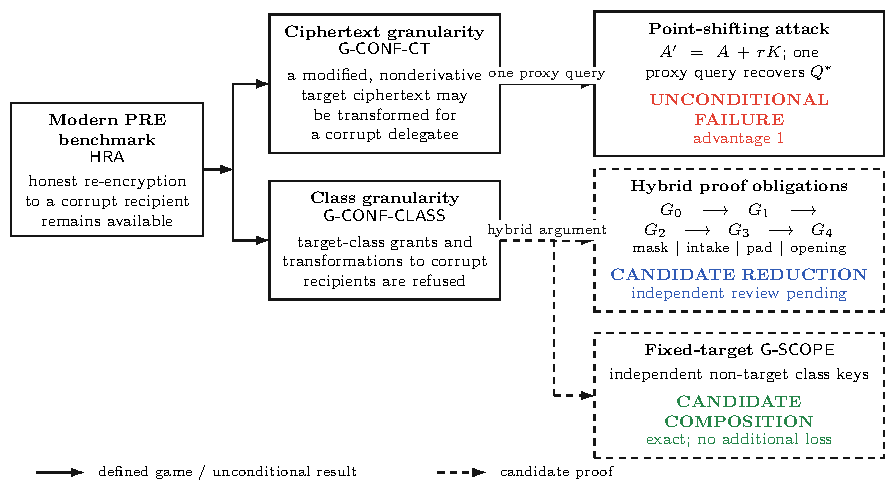
\includegraphics[width=\textwidth]{figures/cipherauth_figure2_game_map.pdf}
\caption{Game map, negative result, and positive proof obligations.  The red
branch is unconditional for the specified construction.  The blue and green
branches remain candidate reductions pending independent cryptographic review.}
\label{fig:game-map}
\end{figure}

\section{Per-ciphertext confidentiality is false}
\label{sec:attack}

\begin{theorem}[Point-shifting attack]
The \CEA comparator fails the per-ciphertext game \GCT.  A corrupted delegatee wins with
probability one, except for validation events that occur with negligible
probability under honest challenge generation.
\end{theorem}

\begin{proof}
Let the challenge contain \(A^*=t^*K\), ciphertext component \(E^*\), and
authenticated commitment \(c^*\).  The adversary chooses known
\(r\in\Zq^*\) and replaces the unsigned point by
\[
 A'=A^*+rK=(t^*+r)K.
\]
It leaves \(\Lambda^*,c^*,E^*\) and the aggregate authentication unchanged.
Public verification still accepts because the signed statement contains \(c^*\),
not \(A^*\).  The submitted core differs from the registered challenge core, so
the \GCT proxy query is allowed.

For the corrupted delegatee's grant, the proxy returns
\[
 \bar A'=\Omega^{-1}A'=\omega^{-1}(Q^*+rP).
\]
The delegatee uses its secret key and the public token to recover \(\omega\),
then computes \(Q'=\omega\bar A'=Q^*+rP\) and
\(Q^*=Q'-rP\).  It decrypts \(E^*\) with \(\KDF(Q^*)\), learning the challenge
bit.  The commitment check succeeds for the recovered challenge message.  No
decryption-oracle query is needed.
\end{proof}

The attack explains why authenticating an invariant commitment is insufficient
for per-ciphertext proxy policy.  A repair must give the proxy a sound way to
validate the relation between \(A\) and the encryption randomness, such as a
proof of knowledge tied to the complete ciphertext.  Whether such proofs can be
compressed while retaining per-record extraction is a separate construction and
proof problem.

\paragraph{In-class collusion.}
The token also makes in-class key recovery explicit.  The proxy knows
\(\Omega=\omega k\), while the delegatee recovers \(\omega\).  Their coalition
computes \(k=\Omega\omega^{-1}\).  Consequently, retained grant material cannot
support revocation within a class and epoch.  Independent future-epoch keys can
limit future access, but they cannot retract access to an old class key.

\section{Candidate class-granular confidentiality theorem}
\label{sec:class-proof}

Define confidentiality advantage as
\(\left|\Pr[b'=b]-\tfrac12\right|\).  Let \(N_H\) be the number of statically
honest delegatees, \(q_{\mathrm{pre}}\) the number of distinct challenge-proof
inputs queried before the challenge proof is installed, \(q_c\) the number of
commitment-oracle queries, and \(Q_D\) the number of record-opening attempts in
ordinary nonrefused decryption queries.

\begin{theorem}[Candidate class-confidentiality bound]
\label{thm:class}
In the random oracle model, under GDivDH, the frozen \GClass-v1 interface satisfies
\begin{align*}
\Adv_{\GClass}(\mathcal A)
\le{}& \Succ_{\mathrm{GDivDH}}(\mathcal B_{\mathrm{chal}})
 + N_H\Succ_{\mathrm{GDivDH}}(\mathcal B_{\mathrm{mask}})\\
&+\frac{q_{\mathrm{pre}}}{q-1}
 +\frac{q_c}{2^\lambda}
 +\frac{Q_D(q_c+1)}{2^\lambda},
\end{align*}
capped at one.  The two GDivDH solvers are distinct reductions.  The statement
assumes static corruption and class-granular confidentiality; authenticity and
concrete-hash analysis are treated separately.
\end{theorem}

\subsection{Hybrid argument}

Game \(G_0\) is the real \GClass-v1 game.  Target-class grants and proxy service
to corrupted recipients are refused.  Proxy outputs to honest delegatees are
registered as derivatives, and decryption refuses registered cores and applies
the \(\TEST\) mask.

In \(G_1\), for every honest target-class grant, replace the following value by
uniform bytes:
\[
 C=\mathsf{enc}(\omega)\oplus\Hmask(T,\KeyRef_K).
\]
Sample
\(\Omega\leftarrow\Zq^*\) directly, set \(W=\HOmega(\Omega)\), and retain
\(\Omega\) at the proxy.  Multiplication by fixed nonzero \(k\) is a bijection,
so \(\Omega\) has its real distribution.  Until the adversary queries the exact
context-bound mask point, the two games are identical.  Section~\ref{sec:mask}
reduces the bad event with loss \(N_H\).  In this hybrid every target-class proxy
reply is exact for arbitrary input:
\[
  \bar A=\Omega^{-1}A.
\]
This step is why no target-record knowledge extractor is needed.

Game \(G_2\) installs a simulated challenge intake proof.  Use the main GDivDH
instance as \(K^*=aP\) and \(A^*=bP\).  Sample a challenge and response
\((c_p,z_p)\), form
\(R^*=z_pK^*-c_pA^*\), reject the identity, and program the exact fresh proof
input to \(c_p\).  Conditioned on freshness, the transcript has the honest
Schnorr distribution.  Each prequeried input fixes at most one encodable
\(R^*\), giving distance at most \(q_{\mathrm{pre}}/(q-1)\).

In \(G_3\), sample the challenge pad, digest \(d^*\), and commitment \(c^*\)
uniformly, and program \(\Hc(m_b,d^*)=c^*\) if fresh.  Until the adversary asks
\(\KDF\) or \(\Hd\) at \(Q^*=(b/a)P\), this has the real challenge
distribution.  The GDivDH decision oracle recognizes a point \(Q\) satisfying
\(A^*=aQ\), after which \(\mathcal B_{\mathrm{chal}}\) outputs \(Q\).  A
commitment prequery hits \((m_b,d^*)\) with probability at most
\(q_c/2^\lambda\).

In \(G_4\), ordinary decryption scans the recorded \(\KDF\) and \(\Hd\) point
queries.  The decision oracle recognizes a candidate \(Q\) satisfying \(A=kQ\).
If found, the simulator completes missing oracle values and verifies the opening.
For a delegated record under an honest target grant, it first restores
\(A=\Omega\bar A\).  If a real opening accepts without the correct point in
either query list, the unseen \(\Hd(Q)\) value must cause an earlier commitment
collision or a fresh \(\lambda\)-bit guess.  The probability is at most
\((q_c+1)/2^\lambda\) per attempt, hence
\(Q_D(q_c+1)/2^\lambda\) in total.

Conditioned on none of these events, the challenge pad and commitment remain
uniform at every allowed interface.  The final view is independent of \(b\).
Summing the game differences gives Theorem~\ref{thm:class}.

\subsection{Mask exposure reduction}
\label{sec:mask}

The reduction guesses one of at most \(N_H\) honest delegatees and publishes its
key as \(U=aP\) from a GDivDH instance \((P,U,V=bP)\).  For the \(j\)-th grant to
that delegatee it samples nonzero \(r_j\) and publishes
\(\gamma_j=r_jV\).  The hidden mask point is
\(T_j=r_j(b/a)P\).  The reduction samples \(C_j\) and \(\Omega_j\) uniformly,
sets \(W_j=\HOmega(\Omega_j)\), signs the public token digest, and answers every
proxy transformation as \(\Omega_j^{-1}A\).

For each context-correct \(\Hmask\) query \(X\), the solver tests every stored
grant with its decision oracle.  It also tests earlier mask queries when a new
grant is installed.  If \(\gamma_j=aX\), then \(X=T_j\), and
\(r_j^{-1}X=(b/a)P\) solves the instance.  No grant index or mask-query index is
guessed; only the honest-delegatee guess contributes loss.  Thus
\[
 \Pr[\mathsf{Bad}_{\mathrm{mask}}]
 \le N_H\Succ_{\mathrm{GDivDH}}(\mathcal B_{\mathrm{mask}}).
\]
Static honesty is essential because later disclosure of \(k_\ell\) would reveal
\(T_j=k_\ell^{-1}\gamma_j\) directly.

\subsection{Why algebraic extraction is absent}

An earlier route attempted to extract a numerical opening from every accepted
compressed intake proof.  That is unnecessary for \GClass.  The only target-class
proxy service is to honest delegatees, and the simulator knows the corresponding
scalar \(\Omega\) after the uniform-mask hybrid.  It can therefore transform any
group point, including the challenge and adversarial affine combinations, without
knowing an opening.  Repeated-query and cross-grant linear relations are preserved
because the simulated map is the real linear map.

For decryption, the GDivDH decision oracle identifies openings already present in
the random-oracle query tables.  A missing point query is accounted for by the
explicit commitment-guessing term.  The aggregate intake equation remains part
of the implemented proxy interface; Theorem~\ref{thm:class} instead relies on
exact scalar simulation and decision-oracle recognition of queried openings.

\section{Out-of-class scope}
\label{sec:scope}

In \GScope-v1, the adversary may receive complete grants and collude with the
proxy and delegatees for every class of the same origin except the phase-zero
target.  Each class is identified by the full origin key reference, tag, and
epoch.

\begin{theorem}[Candidate exact scope composition]
For a target class fixed before key generation,
\[
  \Adv_{\GScope}(\mathcal A)
  \le \Adv_{\GClass}(\mathcal B).
\]
The composition adds no assumption or additive loss.  Substituting
Theorem~\ref{thm:class} gives the same right-hand side.
\end{theorem}

\begin{proof}
The reduction forwards the fixed target class to its class-confidentiality challenger and
generates every other class key independently.  It knows those scalars and answers
non-target grants, token disclosure, proxy corruption, re-encryption, and
decryption exactly, including recovery of a granted non-target class key by a
proxy--delegatee coalition.

Cross-class substitution is rejected by the canonical bindings: sender statements
bind the complete origin key reference, tag, and epoch; grants and token digests
bind the origin and delegatee references and public token fields; the proxy checks
the grant against the aggregate context.  The mask-oracle input also includes the
full origin class reference.  Global \(\KDF\) and \(\Hd\) queries are already
handled by the main class solver.  The simulated view is therefore exact.
\end{proof}

An adaptive target selected after observing \(N\) eligible class keys incurs at
least the elementary random-index factor \(N\) under this reduction.

\section{Authentication, costs, and artifact evidence}
\label{sec:artifact}

Aggregate authentication follows through a reduction in which a fresh
honest-sender statement in an accepted aggregate yields either a chosen-key
IASchnorr forgery or a collision in \(\Hc\).  Grant authenticity reduces to
Schnorr EUF-CMA under identity-authenticated key registration.  The proof ledger
tracks the exact Chen--Zhao loss transcription for the aggregate theorem.

The implemented origin record adds one compressed group point \(\Lambda\) and one
32-byte commitment \(c\) to the hashed-ElGamal core, plus one 32-byte aggregate
response per batch.  The public token contains 97 bytes before framing:
\((C,\gamma,W)\).  In the canonical prototype wire format, an eight-record batch
with 32-byte messages is 1337 bytes at the origin and 1665 bytes after delegation;
the signed grant and public token add 328 bytes.

The artifact contains 286 unique tests: 270 for the current chain and 16 preserved
historical diagnostics.  It also replays 33 deterministic traces and compiles 266
Python files.  The integrated path is
\[
 \text{sender}\to\text{compressed intake}\to\text{proxy}
 \to\text{canonical wire}\to\text{delegatee opening}.
\]
All tests pass with zero failures, errors, or skips.  The source manifest is
checked separately so review material cannot be inserted into the frozen codebase
without detection.

The complete review artifact, including source, tests, and deterministic traces,
is available at \artifacturl.

The test suite covers exact commutation, origin/delegatee opening equality,
canonical serialization, malformed encodings, scope bindings, the \(A\)-mauling
attack, the in-class key-recovery non-goal, token-hybrid algebra, challenge-proof
programming, and the quantitative loss calculator.  These tests validate the
executable and algebraic claims, while the reductions carry the computational
claims.  The machine-readable summary records these evidence classes separately.

\section{Discussion}

The construction exposes a useful distinction between authentication invariance
and proxy-validity.  Signing an invariant commitment is sufficient for exact
aggregate commutation and end-recipient integrity.  It is insufficient when a
proxy must enforce policy at ciphertext granularity, because the proxy cannot open
the commitment.  A proxy-checkable validity proof could close that gap, but then
knowledge soundness and its interaction with aggregation become part of the main
security argument.

Class granularity is coherent only when the deployment accepts its consequences.
A class is an authorization unit rather than metadata alone.  A target class cannot be
served to corrupted recipients, and collusion on a granted class reveals that
class key.  Short epochs and independent keys limit future exposure but do not
provide cryptographic revocation of retained material.

The reductions use the GDivDH decision oracle to detect the challenge opening and
token-mask exposure while retaining the standard DCDH computational target.
Twin-DH techniques offer a concrete route for eliminating decision oracles in
related settings~\cite{CKS08}; adapting that route to the present interface is the
natural next theoretical step.

\section{Conclusion}

Commitment signing makes aggregation and delegation commute, but the same design
leaves the encryption point unchecked at the proxy.  The resulting gap is sharp:
per-ciphertext confidentiality fails by a one-query mauling attack, while a
class-granular notion---strictly weaker than HRA because corrupt target recipients
are refused---admits an exact token simulation and an explicit candidate
reduction.  Independent class keys extend that result to out-of-class collusion
without further loss.  Together, the attack, game separation, candidate
quantitative bound, and exact scope composition define the achieved security
frontier of the comparator.

\appendix
\section{Frozen oracle rules}

For clarity, this appendix records the target-class rules used by the candidate
theorem.  \(\GrantO\) refuses corrupted target-class delegatees.  For an honest
delegatee it returns only the signed grant and public \((C,\gamma,W)\), retaining
\(\Omega\) at the proxy.  \(\ReEncO\) requires a recorded admissible grant and
public/intake acceptance, refuses corrupted target-class delegatees for every
input, and registers outputs derived from a challenge core.  \(\DecO\) first
refuses every registered core or derivative; otherwise it performs ordinary
opening and masks either challenge message with \(\TEST\).  Target-proxy
corruption is unavailable.

The challenge registers \((\KeyRef_K,A^*,E^*)\).  Re-encryption of the exact
challenge to an honest delegatee is allowed and the result becomes a derivative.
This query is simulatable as \(\Omega^{-1}A^*\); no opening of \(A^*\) is needed.

\section{Proof-obligation ledger}

\begin{center}
\textbf{Table 1. Status at the release date.}\par\smallskip
\begin{tabular}{p{0.32\textwidth}p{0.58\textwidth}}
\toprule
Item & Status \\
\midrule
Exact aggregate/delegate commutation & Algebraic identity; tested \\
Per-ciphertext \(A\)-mauling attack & Concrete attack; tested \\
In-class proxy--delegatee key recovery & Algebraic attack; tested \\
\GClass-v1 quantitative bound & Candidate proof; independent review required \\
\GScope-v1 fixed-target composition & Candidate exact composition; independent review required \\
Aggregate sender authenticity & Known-theorem composition sketch; exact loss transcription and review required \\
Grant authenticity & Schnorr reduction sketch; review required \\
Concrete SHA-256 security & Not claimed \\
Machine-checked cryptographic proof & None \\
\bottomrule
\end{tabular}
\end{center}

\bibliographystyle{alpha}
\bibliography{references}

\end{document}
